% ============================================================
%  يُترجَم بـ XeLaTeX  (في Overleaf: Menu → Compiler → XeLaTeX)
%  الخط: Amiri (متوفر في Overleaf، أو حمّله من github.com/aliftype/amiri)
% ============================================================
\documentclass[12pt,a4paper]{article}
\usepackage[a4paper,margin=1.7cm,top=2.3cm,bottom=2.9cm,headheight=15pt,footskip=1.5cm]{geometry}
\usepackage{amsmath,amssymb}
\usepackage{icomma}
\usepackage[english,bidi=default,layout=lists]{babel}
\babelprovide[import,main]{arabic}
\babelfont{rm}[Scale=1.08]{Amiri}
\babelfont{sf}[Scale=1.08]{Amiri}
\usepackage[most]{tcolorbox}
\usepackage{tikz}
\usetikzlibrary{arrows.meta,calc,shadings}
\usepackage{array}
\usepackage{colortbl}
\usepackage{fancyhdr}
\usepackage{titlesec}
\usepackage{enumitem}
\usepackage{collcell}
\usepackage{needspace}
\usepackage{etoolbox}
% أعمدة جداول تُكتب خلاياها بالعربية في الاتجاه الصحيح
\newcolumntype{C}{>{\collectcell\ar}c<{\endcollectcell}}
% تجنب عنوان يتيم في أسفل الصفحة
\pretocmd{\section}{\Needspace{15\baselineskip}}{}{}
\pretocmd{\subsection}{\Needspace{11\baselineskip}}{}{}

% ---------- الألوان ----------
\definecolor{cDef}{HTML}{1F4E9C}
\definecolor{cThm}{HTML}{B3261E}
\definecolor{cRem}{HTML}{2E7D32}
\definecolor{cEx}{HTML}{C76B00}
\definecolor{cMeth}{HTML}{6A1B9A}
\definecolor{cSol}{HTML}{00695C}
\definecolor{cSec}{HTML}{1F3A68}

% ---------- العناوين ----------
\titleformat{\section}{\Large\bfseries\color{cSec}}{\thesection.}{0.6em}{}[{\color{cSec!60}\titlerule[1pt]}]
\titleformat{\subsection}{\large\bfseries\color{cThm!85!black}}{\thesubsection.}{0.5em}{}
\titlespacing*{\section}{0pt}{14pt}{8pt}
\titlespacing*{\subsection}{0pt}{10pt}{5pt}
\setlength{\parindent}{0pt}
\setlength{\parskip}{4pt}
\setlist{itemsep=2pt,topsep=3pt}

% ---------- الصناديق (تُرسم في سياق LTR ويُكتب محتواها بالعربية) ----------
\newtcolorbox{arbox}[3][]{enhanced,
  colback=#2!5,colframe=#2!80!black,arc=2mm,boxrule=0.8pt,
  left=6pt,right=6pt,top=8pt,bottom=5pt,
  fonttitle=\bfseries,coltitle=white,
  title={\foreignlanguage{arabic}{#3}},
  attach boxed title to top right={xshift=-5mm,yshift=-3mm},
  boxed title style={colback=#2!80!black,arc=1.5mm,boxrule=0pt},
  before upper={\selectlanguage{arabic}},
  before skip=8pt,after skip=8pt,breakable,#1}
\newenvironment{BOX}[2]{\begin{otherlanguage}{english}\begin{arbox}{#1}{#2}}{\end{arbox}\end{otherlanguage}}
\newenvironment{tarif}[1][تعريف]{\begin{BOX}{cDef}{#1}}{\end{BOX}}
\newenvironment{khassia}[1][خاصية]{\begin{BOX}{cThm}{#1}}{\end{BOX}}
\newenvironment{molahada}[1][ملاحظة]{\begin{BOX}{cRem}{#1}}{\end{BOX}}
\newenvironment{mithal}[1][مثال]{\begin{BOX}{cEx}{#1}}{\end{BOX}}
\newenvironment{tariqa}[1][طريقة]{\begin{BOX}{cMeth}{#1}}{\end{BOX}}

% ---------- التمارين والحلول ----------
\newcounter{exo}
\newenvironment{tamrin}[1]{\stepcounter{exo}\begin{BOX}{cSec}{التمرين \theexo: #1}}{\end{BOX}}
\newenvironment{hal}{\Needspace{12\baselineskip}\begin{otherlanguage}{english}\begin{arbox}[breakable]{cSol}{حل التمرين \theexo}}{\end{arbox}\end{otherlanguage}}

% رسومات TikZ تُوضع في سياق LTR
\newenvironment{LTR}{\begin{otherlanguage}{english}}{\end{otherlanguage}}
\newcommand{\ar}[1]{\foreignlanguage{arabic}{#1}}

% ---------- رموز ----------
% نقاط الحذف داخل الرياضيات (\dots يسبب خللاً في الاتجاه مع babel)
\renewcommand{\dots}{\mathinner{\ldotp\ldotp\ldotp}}
\renewcommand{\ldots}{\mathinner{\ldotp\ldotp\ldotp}}
\renewcommand{\cdots}{\mathinner{\cdotp\cdotp\cdotp}}
\newcommand{\N}{\mathbb{N}}
\newcommand{\Z}{\mathbb{Z}}
\newcommand{\D}{\mathbb{D}}
\newcommand{\Q}{\mathbb{Q}}
\newcommand{\R}{\mathbb{R}}
\newcommand{\pgcd}{\operatorname{PGCD}}
\newcommand{\ppcm}{\operatorname{PPCM}}

% ---------- تمثيل مجال على مستقيم عددي ----------
% \NLseg{a}{b}{[}{]}  مجال محدود
\newcommand{\NLseg}[4]{\begin{LTR}\begin{tikzpicture}[baseline=-0.6ex]
 \draw[-{Stealth[length=2mm]},gray!70](0,0)--(3.4,0);
 \draw[line width=2pt,cThm!80!black](0.7,0)--(2.7,0);
 \node[cThm!80!black,font=\LARGE] at (0.7,0){$#3$};
 \node[cThm!80!black,font=\LARGE] at (2.7,0){$#4$};
 \node[below=3pt,font=\footnotesize] at (0.7,0){$#1$};
 \node[below=3pt,font=\footnotesize] at (2.7,0){$#2$};
\end{tikzpicture}\end{LTR}}
% \NLright{a}{[}  مجال نحو +∞
\newcommand{\NLright}[2]{\begin{LTR}\begin{tikzpicture}[baseline=-0.6ex]
 \draw[-{Stealth[length=2mm]},gray!70](0,0)--(3.4,0);
 \draw[line width=2pt,cThm!80!black](1.3,0)--(3.3,0);
 \node[cThm!80!black,font=\LARGE] at (1.3,0){$#2$};
 \node[below=3pt,font=\footnotesize] at (1.3,0){$#1$};
\end{tikzpicture}\end{LTR}}
% \NLleft{b}{]}  مجال نحو −∞
\newcommand{\NLleft}[2]{\begin{LTR}\begin{tikzpicture}[baseline=-0.6ex]
 \draw[-{Stealth[length=2mm]},gray!70](0,0)--(3.4,0);
 \draw[line width=2pt,cThm!80!black](0.05,0)--(2.1,0);
 \node[cThm!80!black,font=\LARGE] at (2.1,0){$#2$};
 \node[below=3pt,font=\footnotesize] at (2.1,0){$#1$};
\end{tikzpicture}\end{LTR}}

% ---------- أيقونات مواقع التواصل (مرسومة بـ TikZ، لا تحتاج أي حزمة) ----------
\definecolor{cFB}{HTML}{1877F2}
\definecolor{cTG}{HTML}{229ED9}
\definecolor{cIG1}{HTML}{FEDA75}
\definecolor{cIG2}{HTML}{D62976}
\definecolor{cIG3}{HTML}{4F5BD5}
\newcommand{\fbicon}{\begin{LTR}\begin{tikzpicture}[baseline=-0.75ex,x=1em,y=1em]
 \fill[cFB] (0,0) circle (0.55);
 \node[white,inner sep=0,font=\usefont{TU}{lmss}{bx}{n}\small] at (0.04,-0.02) {f};
\end{tikzpicture}\end{LTR}}
\newcommand{\igicon}{\begin{LTR}
\begin{tikzpicture}[baseline=-0.75ex,x=1em,y=1em]
 \shade[lower left=cIG1,lower right=cIG2,upper left=cIG2,upper right=cIG3,rounded corners=0.28em] (-0.55,-0.55) rectangle (0.55,0.55);
 \draw[white,line width=0.09em,rounded corners=0.18em] (-0.36,-0.36) rectangle (0.36,0.36);
 \draw[white,line width=0.09em] (0,0) circle (0.17);
 \fill[white] (0.22,0.22) circle (0.05);
\end{tikzpicture}\end{LTR}}
\newcommand{\tgicon}{\begin{LTR}
\begin{tikzpicture}[baseline=-0.75ex,x=1em,y=1em]
 \fill[cTG] (0,0) circle (0.55);
 \fill[white] (-0.33,0.0) -- (0.32,0.27) -- (0.2,-0.3) -- (0.0,-0.15) -- (-0.08,-0.28) -- (-0.08,-0.08) -- cycle;
 \fill[cTG!70!black] (-0.08,-0.08) -- (0.25,0.2) -- (0.0,-0.15) -- (-0.08,-0.28) -- cycle;
\end{tikzpicture}\end{LTR}}
% سطر مواقع التواصل أسفل كل صفحة
% (يُكتب السطر بترتيب بصري من اليسار إلى اليمين: الأيقونة يمين كل اسم)
\newcommand{\PageBox}{\begin{LTR}\tikz[baseline=(p.base)]\node[fill=black,text=white,inner sep=2.5pt,minimum width=1.6em,minimum height=1.3em,font=\usefont{TU}{lmss}{bx}{n}\small](p){\ifnum\value{page}<10 0\fi\arabic{page}};\end{LTR}}
\newcommand{\SocialRow}{\begin{otherlanguage}{english}%
 \ar{\textbf{الأستاذ سوايسية هشام للرياضيات}}\ \tgicon\hfill
 \textbf{prof\_hicham\_math}\ \igicon\hfill
 \ar{\textbf{الأستاذ سوايسية هشام للرياضيات}}\ \fbicon\hspace{2.2em}\PageBox\end{otherlanguage}}
% ---------- رأس وتذييل الصفحة ----------
\pagestyle{fancy}
\fancyhf{}
\renewcommand{\headrulewidth}{0.6pt}
\renewcommand{\footrulewidth}{0.4pt}
% \SetHeader{يمين الرأس}{يسار الرأس}{يمين التذييل}{يسار التذييل}
\newcommand{\SetHeader}[2]{%
 \fancyhead[C]{\parbox{\textwidth}{\ar{#1\hfill #2}}}%
 \fancyfoot[C]{\parbox{\textwidth}{\small\SocialRow}}}

\usepackage{tkz-tab}
\usepackage{multicol}
% جدول تغيرات / إشارة (يُرسم في سياق LTR)
\newenvironment{TAB}{\par\begin{center}\begin{LTR}\begin{tikzpicture}[scale=0.95,every node/.style={font=\small}]}{\end{tikzpicture}\end{LTR}\end{center}}
% معلم بشبكة: \begin{GR}{xmin}{xmax}{ymin}{ymax}{unit cm}
\newenvironment{GR}[5]{\par\begin{center}\begin{LTR}\begin{tikzpicture}[x=#5cm,y=#5cm,font=\footnotesize]
 \def\xmn{#1}\def\xmx{#2}\def\ymn{#3}\def\ymx{#4}
 \draw[gray!25,very thin] (#1,#3) grid (#2,#4);
 \draw[-{Stealth[length=2mm]}] (#1,0)--(#2+0.3,0) node[below left]{$x$};
 \draw[-{Stealth[length=2mm]}] (0,#3)--(0,#4+0.3) node[below left]{$y$};
 \node[below left] at (0,0){$O$};
 \draw[very thick,-{Stealth[length=1.6mm]}] (0,0)--(1,0) node[below,pos=.55]{$\vec i$};
 \draw[very thick,-{Stealth[length=1.6mm]}] (0,0)--(0,1) node[left,pos=.55]{$\vec j$};
 \begin{scope}\clip (#1,#3) rectangle (#2,#4);}
{\end{scope}\end{tikzpicture}\end{LTR}\end{center}}
\newcommand{\Ticks}[2]{\foreach \t in {#1} \node[below,font=\scriptsize] at (\t,0){$\t$}; \foreach \t in {#2} \node[left,font=\scriptsize] at (0,\t){$\t$};}
\newcommand{\bx}[1]{\ensuremath{\colorbox{cDef!12}{$\displaystyle #1$}}}
\newcommand{\hl}[1]{\ensuremath{\colorbox{cEx!20}{$\displaystyle #1$}}}
\newcommand{\Lim}[1]{\displaystyle\lim_{x\to #1}}
\newcommand{\Cf}{(C_f)}
\newenvironment{qst}{\begin{enumerate}[label=\protect\circled{\arabic*},leftmargin=*]}{\end{enumerate}}
\newcommand{\circled}[1]{\foreignlanguage{english}{\tikz[baseline=(c.base)]\node[circle,fill=cDef,text=white,inner sep=1.2pt,font=\scriptsize\bfseries](c){#1};}}
% عمودان: \TwoCol{عرض اليسار}{محتوى اليسار}{عرض اليمين}{محتوى اليمين}  (آمن مع TikZ)
\newcommand{\TwoCol}[4]{\par\begin{LTR}\noindent\begin{minipage}[t]{#1\textwidth}\selectlanguage{arabic}#2\end{minipage}\hfill\begin{minipage}[t]{#3\textwidth}\selectlanguage{arabic}#4\end{minipage}\end{LTR}\par}
\newcommand{\un}{(u_n)}\newcommand{\vn}{(v_n)}
% برهان بالتراجع: \Rec{الخاصية P(n)}{التحقق من P(0)}{البرهان على الوراثة}
\newcommand{\Rec}[3]{\textbf{برهان بالتراجع:} نسمي $P(n)$ الخاصية: «#1».
\begin{itemize}
\item \textbf{التحقق:} #2
\item \textbf{الوراثة:} نفرض أن $P(n)$ صحيحة ونبرهن صحة $P(n+1)$: #3
\item \textbf{الخلاصة:} حسب مبدأ الاستدلال بالتراجع، $P(n)$ صحيحة من أجل كل عدد طبيعي $n$.
\end{itemize}}
\newcommand{\src}[1]{{\footnotesize\textbf{#1}}\par}
\newcommand{\ok}{$\textcolor{cRem}{\checkmark}$}
\newcommand{\limn}{\displaystyle\lim_{n\to+\infty}}
% أسئلة فرعية (أ) (ب) (جـ) كل سؤال في سطر
\newenvironment{sq}{\begin{itemize}[leftmargin=2.4em,itemsep=3pt]}{\end{itemize}}
\newcommand{\qa}{\item[(أ)]}\newcommand{\qb}{\item[(ب)]}\newcommand{\qc}{\item[(جـ)]}\newcommand{\qd}{\item[(د)]}\newcommand{\qe}{\item[(هـ)]}
\newcommand{\pa}{\par\smallskip\textbf{(أ)} }\newcommand{\pb}{\par\smallskip\textbf{(ب)} }\newcommand{\pc}{\par\smallskip\textbf{(جـ)} }\newcommand{\pd}{\par\smallskip\textbf{(د)} }\newcommand{\pe}{\par\smallskip\textbf{(هـ)} }
\newcommand{\ccl}[1]{\par\textbf{الخلاصة:} #1}

\pretocmd{\section}{\Needspace{24\baselineskip}}{}{}
\SetHeader{\small\bfseries\color{cSec}تمارين: المرجح في المستوي}{\small\color{cSec}السنة الثانية ثانوي -- الشعب العلمية}
\begin{document}
\newcolumntype{M}[1]{>{\centering\arraybackslash}p{#1}}
\newcommand{\RL}[4]{\TwoCol{#3}{#4}{#1}{#2}}
\newcommand{\QQ}[1]{\par\smallskip\textbf{#1.} }
\newcommand{\V}[1]{\overrightarrow{#1}}
\newcommand{\nV}[1]{\big\|#1\big\|}
\newcommand{\ABC}[3]{\\[2pt]\begin{tabular}{p{0.28\textwidth}p{0.28\textwidth}p{0.28\textwidth}}(جـ) \ #3 & (ب) \ #2 & (أ) \ #1\end{tabular}}
\begin{LTR}
\begin{tcolorbox}[enhanced,colback=cSec,colframe=cSec,arc=3mm,halign=center,boxrule=0pt,top=12pt,bottom=12pt,before upper={\selectlanguage{arabic}}]
{\color{white}\fontsize{26}{32}\selectfont\bfseries سلسلة تمارين: المُرَجِّح في المستوي}\\[8pt]
{\color{white}\large تمارين متنوعة ومسائل شاملة مع الحلول المفصلة خطوة بخطوة}\\[5pt]
{\color{white}\large السنة الثانية ثانوي -- الشعب العلمية}
\end{tcolorbox}
\end{LTR}

% =====================================================================
\section{مرجح نقطتين}
% ------------------------------------------------- 1
\begin{tamrin}{تعيين وإنشاء مرجح نقطتين}
$A$ و $B$ نقطتان متمايزتان من المستوي حيث $AB=6\ \text{cm}$.
\begin{enumerate}
\item أنشئ النقطة $G$ مرجح الجملة المثقلة $\{(A;2);(B;3)\}$.
\item أنشئ النقطة $N$ مرجح الجملة المثقلة $\{(A;-3);(B;1)\}$.
\item لتكن $K$ النقطة حيث $\V{BK}=-\dfrac12\V{AK}$. أثبت أن $K$ مرجح النقطتين $A$ و $B$ بمعاملين يطلب تعيينهما.
\item هل يوجد مرجح للجملة $\{(A;5);(B;-5)\}$؟ علّل.
\end{enumerate}
\end{tamrin}
\begin{hal}
\textbf{1.} $2+3=5\ne0$ ، فالمرجح $G$ موجود ووحيد ، و: \ $\V{AG}=\dfrac{3}{2+3}\V{AB}=\bx{\dfrac35\V{AB}}$.\par
$AG=\dfrac35\times6=3{,}6\ \text{cm}$ ، و $G\in[AB]$ (المعاملان موجبان).

\QQ{2} $-3+1=-2\ne0$: \ $\V{AN}=\dfrac{1}{-2}\V{AB}=\bx{-\dfrac12\V{AB}}$. \ $N$ خارج $[AB]$ من جهة $A$ ، و $AN=3\ \text{cm}$.
\begin{center}\begin{LTR}
\begin{tikzpicture}[x=0.8cm,font=\small]
\draw[gray] (-4,0)--(7,0);
\foreach \x in {-3,...,6} \draw (\x,0.07)--(\x,-0.07);
\fill (0,0) circle(1.8pt) node[above]{$A$}; \fill (6,0) circle(1.8pt) node[above]{$B$};
\fill[cThm] (3.6,0) circle(2pt) node[above]{$G$};
\fill[cDef] (-3,0) circle(2pt) node[above]{$N$};
\fill[cEx] (-6,0) circle(0pt);
\end{tikzpicture}
\end{LTR}\end{center}

\QQ{3} $\V{BK}=-\dfrac12\V{AK}$ تكافئ $2\V{BK}+\V{AK}=\vec0$ ، أي (بالضرب في $-1$): \ $\V{KA}+2\V{KB}=\vec0$.\par
إذن \bx{K\ \text{\ar{مرجح}}\ \{(A;1);(B;2)\}} \ ، و $\V{AK}=\dfrac23\V{AB}$ ($AK=4\ \text{cm}$).

\QQ{4} \textbf{لا:} مجموع المعاملين $5+(-5)=0$. \ العلاقة $5\V{GA}-5\V{GB}=\vec0$ تعني $5\V{BA}=\vec0$ ، أي $A=B$ ، وهذا مستحيل.
\end{hal}

% ------------------------------------------------- 2
\begin{tamrin}{علاقة شعاعية وتعيين المعاملات}
$A$ و $B$ نقطتان متمايزتان.
\begin{enumerate}
\item لتكن $G$ نقطة حيث $\V{AG}=\dfrac{3}{10}\V{AB}$. عيّن عددين حقيقيين $m_A$ و $m_B$ حتى تكون $G$ مرجح $\{(A;m_A);(B;m_B)\}$.
\item لتكن $I$ النقطة حيث $\V{AI}=\dfrac43\V{AB}$. بيّن أن $I$ مرجح النقطتين $A$ و $B$ ، ثم عيّن المعاملين.
\item بيّن أنه من أجل كل نقطة $M$: $\V{MA}+3\V{MB}=4\V{MJ}$ حيث $J$ نقطة يطلب تعيينها.
\end{enumerate}
\end{tamrin}
\begin{hal}
\textbf{1.} نبحث عن $m_A$ و $m_B$ حيث $\dfrac{m_B}{m_A+m_B}=\dfrac{3}{10}$. \ نأخذ $m_A+m_B=10$ و $m_B=3$ ، أي $m_A=7$.\par
\textbf{تحقق:} $\V{AG}=\dfrac{3}{10}\V{AB}$ تكافئ $10\V{AG}=3\big(\V{AG}+\V{GB}\big)$ ، أي $7\V{AG}-3\V{GB}=\vec0$ ، أي $7\V{GA}+3\V{GB}=\vec0$: \ \bx{G\ \text{\ar{مرجح}}\ \{(A;7);(B;3)\}}.\par
(وكل جملة $\{(A;7k);(B;3k)\}$ مع $k\ne0$ مناسبة.)

\QQ{2} $3\V{AI}=4\V{AB}=4\big(\V{AI}+\V{IB}\big)$ ، ومنه $-\V{AI}-4\V{IB}=\vec0$ ، أي $\V{IA}-4\V{IB}=\vec0$:\par
\bx{I\ \text{\ar{مرجح}}\ \{(A;1);(B;-4)\}}. \ (تحقق: $\dfrac{-4}{1-4}=\dfrac43$ \ok.)

\QQ{3} $1+3=4\ne0$: نسمي $J$ مرجح $\{(A;1);(B;3)\}$ ، فحسب خاصية الاختزال: $\V{MA}+3\V{MB}=4\V{MJ}$ ، حيث \bx{\V{AJ}=\dfrac34\V{AB}}.
\end{hal}

% =====================================================================
\section{مرجح ثلاث نقط وخاصية التجميع}
% ------------------------------------------------- 3
\begin{tamrin}{إنشاء مرجح ثلاث نقط بطريقتين}
$ABC$ مثلث ، و $G$ مرجح الجملة المثقلة $\{(A;2);(B;3);(C;1)\}$.
\begin{enumerate}
\item عبّر عن $\V{AG}$ بدلالة $\V{AB}$ و $\V{AC}$ ، ثم أنشئ النقطة $G$.
\item لتكن $I$ مرجح $\{(A;2);(B;3)\}$. بيّن أن $G$ مرجح $\{(I;5);(C;1)\}$ ، واستنتج طريقة ثانية لإنشاء $G$.
\item بيّن أنه من أجل كل نقطة $M$: \ $2\V{MA}+3\V{MB}-\V{MC}=4\V{MH}$ حيث $H$ نقطة يطلب تعيينها ، ثم استنتج أن $H$ مرجح $\{(I;5);(C;-1)\}$.
\end{enumerate}
\end{tamrin}
\begin{hal}
\textbf{1.} $2+3+1=6\ne0$: \ $\V{AG}=\dfrac36\V{AB}+\dfrac16\V{AC}=\bx{\dfrac12\V{AB}+\dfrac16\V{AC}}$.\par
\textbf{الإنشاء:} $K$ منتصف $[AB]$ ، و $L$ حيث $\V{AL}=\dfrac16\V{AC}$ ، و $G$ الرأس الرابع لمتوازي الأضلاع $AKGL$.

\QQ{2} $I$ مرجح $\{(A;2);(B;3)\}$: $\V{AI}=\dfrac35\V{AB}$. \ حسب خاصية التجميع: \bx{G\ \text{\ar{مرجح}}\ \{(I;5);(C;1)\}}.\par
ومنه $\V{IG}=\dfrac{1}{5+1}\V{IC}=\bx{\dfrac16\V{IC}}$: \ ننشئ $I$ على $[AB]$ ثم $G$ على $[IC]$ عند سدسها انطلاقاً من $I$.
\begin{center}\begin{LTR}
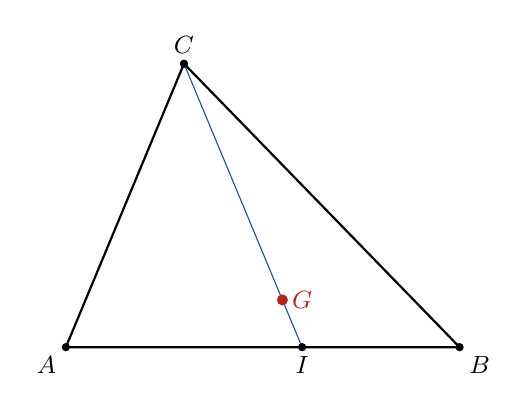
\begin{tikzpicture}[scale=1,font=\small]
\coordinate (A) at (0,0); \coordinate (B) at (5,0); \coordinate (C) at (1.5,3.6);
\coordinate (I) at (3,0); \coordinate (G) at (2.75,0.6);
\draw[thick] (A)--(B)--(C)--cycle; \draw[cDef] (I)--(C);
\fill (A) circle(1.5pt) node[below left]{$A$}; \fill (B) circle(1.5pt) node[below right]{$B$};
\fill (C) circle(1.5pt) node[above]{$C$}; \fill (I) circle(1.5pt) node[below]{$I$};
\fill[cThm] (G) circle(2pt) node[right]{$G$};
\end{tikzpicture}
\end{LTR}\end{center}

\QQ{3} $2+3-1=4\ne0$: نسمي $H$ مرجح $\{(A;2);(B;3);(C;-1)\}$ ، فبالاختزال: $2\V{MA}+3\V{MB}-\V{MC}=4\V{MH}$.\par
بالتجميع ($\{(A;2);(B;3)\}$ مرجحها $I$): \ \bx{H\ \text{\ar{مرجح}}\ \{(I;5);(C;-1)\}} \ ، و $\V{IH}=\dfrac{-1}{4}\V{IC}$.
\end{hal}

% ------------------------------------------------- 4
\begin{tamrin}{خاصية التجميع ومنتصف قطعة}
$ABC$ مثلث كيفي. $H$ نقطة تحقق العلاقة: $2\V{AH}+\V{AB}=\vec0$ ، و $G$ مرجح الجملة المثقلة $\{(A;3);(B;-1);(C;2)\}$.
\begin{enumerate}
\item بيّن أن $H$ هي مرجح النقطتين $A$ و $B$ المرفقتين على الترتيب بمعاملين يطلب تعيينهما.
\item عيّن ثم أنشئ النقطتين $H$ و $G$.
\item اعتماداً على خاصية التجميع أثبت أن $G$ منتصف القطعة المستقيمة $[HC]$.
\item $(E)$ مجموعة النقط $M$ من المستوي حيث: $\nV{3\V{MA}-\V{MB}+2\V{MC}}\le2\nV{\V{MA}-\V{MB}}$. \ عيّن ثم أنشئ المجموعة $(E)$.
\end{enumerate}
\end{tamrin}
\begin{hal}
\textbf{1.} $2\V{AH}+\big(\V{AH}+\V{HB}\big)=\vec0$ ، أي $3\V{AH}+\V{HB}=\vec0$ ، أي $-3\V{HA}+\V{HB}=\vec0$ ، وبالضرب في $-1$: $3\V{HA}-\V{HB}=\vec0$.\par
إذن \bx{H\ \text{\ar{مرجح}}\ \{(A;3);(B;-1)\}}.

\QQ{2} $\V{AH}=-\dfrac12\V{AB}$: $H$ نظيرة منتصف $[AB]$ بالنسبة لـ $A$ (خارج $[AB]$ من جهة $A$).\par
$3-1+2=4\ne0$: \ $\V{AG}=\dfrac{-1}{4}\V{AB}+\dfrac24\V{AC}=-\dfrac14\V{AB}+\dfrac12\V{AC}$.

\QQ{3} $H$ مرجح $\{(A;3);(B;-1)\}$ (مجموع معاملاتها $2$) ، فحسب خاصية التجميع: $G$ مرجح $\{(H;2);(C;2)\}$.\par
المعاملان متساويان ، إذن \bx{G\ \text{\ar{منتصف}}\ [HC]}. \ (تحقق: $\V{AG}=\dfrac12\big(\V{AH}+\V{AC}\big)=-\dfrac14\V{AB}+\dfrac12\V{AC}$ \ok.)

\QQ{4} $3\V{MA}-\V{MB}+2\V{MC}=4\V{MG}$ ، و $\V{MA}-\V{MB}=\V{BA}$ (شعاع ثابت).\par
الشرط يصبح: $4MG\le2AB$ ، أي $MG\le\dfrac{AB}{2}$: \ $(E)$ هي \bx{\text{\ar{القرص الذي مركزه}}\ G\ \text{\ar{ونصف قطره}}\ \dfrac{AB}{2}} (الدائرة وداخلها).
\end{hal}

% ------------------------------------------------- 5
\begin{tamrin}{تجميع بمعاملات سالبة}
$ABC$ مثلث ، و $G$ مرجح الجملة المثقلة $\{(A;-2);(B;1);(C;3)\}$.
\begin{enumerate}
\item أنشئ النقطة $G'$ مرجح الجملة المثقلة $\{(B;1);(C;3)\}$.
\item برهن أن $G$ مرجح الجملة المثقلة $\{(A;-2);(G';4)\}$.
\item أنشئ النقطة $G$.
\end{enumerate}
\end{tamrin}
\begin{hal}
\textbf{1.} $1+3=4\ne0$: \ \bx{\V{BG'}=\dfrac34\V{BC}}.
\QQ{2} $-2+1+3=2\ne0$ فالمرجح $G$ موجود. \ $\{(B;1);(C;3)\}$ مرجحها $G'$ ومجموع معاملاتها $4$. \ حسب خاصية التجميع: \bx{G\ \text{\ar{مرجح}}\ \{(A;-2);(G';4)\}}.
\QQ{3} $\V{AG}=\dfrac{4}{-2+4}\V{AG'}=\bx{2\V{AG'}}$: \ $G$ نظيرة $A$ بالنسبة لـ $G'$ ($G'$ منتصف $[AG]$).
\begin{center}\begin{LTR}
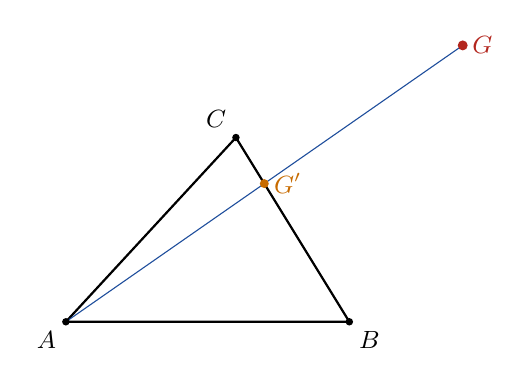
\begin{tikzpicture}[scale=0.9,font=\small]
\coordinate (A) at (0,0); \coordinate (B) at (4,0); \coordinate (C) at (2.4,2.6);
\coordinate (G1) at (2.8,1.95); \coordinate (G) at (5.6,3.9);
\draw[thick] (A)--(B)--(C)--cycle; \draw[cDef] (A)--(G);
\fill (A) circle(1.5pt) node[below left]{$A$}; \fill (B) circle(1.5pt) node[below right]{$B$};
\fill (C) circle(1.5pt) node[above left]{$C$}; \fill[cEx] (G1) circle(1.8pt) node[right]{$G'$};
\fill[cThm] (G) circle(2pt) node[right]{$G$};
\end{tikzpicture}
\end{LTR}\end{center}
\end{hal}

% =====================================================================
\section{إحداثيا المرجح}
% ------------------------------------------------- 6
\begin{tamrin}{إحداثيات ومتوازي أضلاع}
في المستوي المنسوب إلى المعلم المتعامد والمتجانس $(O;\vec i,\vec j)$ ، نعتبر النقط: $A(1;0)$ ، $B(-3;2)$ و $C(1;3)$. \ ولتكن $G$ مرجح الجملة المثقلة $\{(A;-2);(B;1);(C;-1)\}$.
\begin{enumerate}
\item عيّن إحداثيي النقطة $G$.
\item عيّن إحداثيي النقطة $D$ حتى يكون الرباعي $ABCD$ متوازي أضلاع.
\item عيّن الأعداد الحقيقية $\alpha$ ، $\beta$ و $\gamma$ حتى تكون النقطة $D$ مرجح الجملة $\{(A;\alpha);(B;\beta);(C;\gamma)\}$.
\item عيّن $(\Gamma)$ مجموعة النقط $M$ من المستوي حيث: $\nV{-2\V{MA}+\V{MB}-\V{MC}}=2\nV{\V{MA}-\V{MB}+\V{MC}}$.
\end{enumerate}
\end{tamrin}
\begin{hal}
\textbf{1.} $-2+1-1=-2\ne0$:
\[x_G=\frac{-2(1)+1(-3)-1(1)}{-2}=\frac{-6}{-2}=3\qquad;\qquad y_G=\frac{-2(0)+1(2)-1(3)}{-2}=\frac{-1}{-2}=\frac12 .\]
\bx{G\Big(3;\dfrac12\Big)}.

\QQ{2} $ABCD$ متوازي أضلاع $\iff\V{AB}=\V{DC}$: \ $\V{AB}(-4;2)$ و $\V{DC}(1-x_D;3-y_D)$.\par
$1-x_D=-4$ و $3-y_D=2$ ، ومنه \bx{D(5;1)}.

\QQ{3} $\V{AB}=\V{DC}$ تكافئ $\V{DB}-\V{DA}=\V{DC}$ ، أي $\V{DA}-\V{DB}+\V{DC}=\vec0$: \ \bx{\alpha=1\ ،\ \beta=-1\ ،\ \gamma=1} (أو كل مضاعف غير معدوم لها).\par
\textbf{تحقق:} $x=\dfrac{1+3+1}{1}=5$ ، $y=\dfrac{0-2+3}{1}=1$ \ok.

\QQ{4} $-2\V{MA}+\V{MB}-\V{MC}=-2\V{MG}$ ، و $\V{MA}-\V{MB}+\V{MC}=1\times\V{MD}$ (مجموع المعاملات $1$).\par
الشرط: $2MG=2MD$ ، أي $MG=MD$: \ $(\Gamma)$ هي \bx{\text{\ar{محور القطعة}}\ [GD]}.
\end{hal}

% ------------------------------------------------- 7
\begin{tamrin}{مرجح بوسيط ومحل هندسي}
في المستوي المنسوب إلى المعلم المتعامد والمتجانس $(O;\vec i,\vec j)$ ، نعتبر النقط $A(0;1)$ ، $B(0;5)$ و $C(2;1)$. \ لتكن $G_m$ مرجح الجملة المثقلة $\{(A;-m^2+4);(B;m^2-2m);(C;2m)\}$ حيث $m$ عدد حقيقي.
\begin{enumerate}
\item عيّن قيم $m$ التي من أجلها تكون $G_m$ موجودة ووحيدة.
\item عيّن إحداثيي النقطة $G_m$ بدلالة $m$.
\item ما هو المحل الهندسي للنقطة $G_m$ لما $m$ يمسح $\R$؟
\end{enumerate}
\end{tamrin}
\begin{hal}
\textbf{1.} مجموع المعاملات: $-m^2+4+m^2-2m+2m=4\ne0$ \ من أجل كل $m$: \ $G_m$ موجودة ووحيدة \bx{\text{\ar{من أجل كل}}\ m\in\R}.

\QQ{2} \[x_{G_m}=\frac{0\times(-m^2+4)+0\times(m^2-2m)+2\times2m}{4}=\frac{4m}{4}=m ,\]
\[y_{G_m}=\frac{1\times(-m^2+4)+5(m^2-2m)+1\times2m}{4}=\frac{4m^2-8m+4}{4}=m^2-2m+1 .\]
\bx{G_m\big(m;\,m^2-2m+1\big)}.

\QQ{3} $x=m$ و $y=m^2-2m+1=x^2-2x+1=(x-1)^2$. \ لما $m$ يمسح $\R$ فإن $x$ يمسح $\R$:\par
المحل الهندسي لـ $G_m$ هو \bx{\text{\ar{القطع المكافئ الذي معادلته}}\ y=(x-1)^2} (التمثيل البياني لدالة مرجعية مزاحة).
\end{hal}

% ------------------------------------------------- 8
\begin{tamrin}{استقامية ومجموعات نقط بالإحداثيات}
في المستوي المنسوب إلى المعلم المتعامد والمتجانس $(O;\vec i,\vec j)$ ، نعتبر النقط $A(1;2)$ ، $B(-8;-1)$ و $C(3;4)$ ، والنقطة $H$ المعرفة بالعلاقة $\V{AH}=\dfrac32\V{AC}$.
\begin{enumerate}
\item بيّن أن $H$ مرجح النقطتين $A$ و $C$ بمعاملين صحيحين يطلب تعيينهما ، ثم عيّن إحداثيي $H$.
\item عيّن إحداثيي النقطة $G$ مرجح الجملة المثقلة $\{(A;1);(B;-1);(C;-3)\}$.
\item بيّن أن النقط $B$ ، $H$ و $G$ على استقامة واحدة.
\item عيّن وأنشئ المجموعة $(E_1)$ للنقط $M$ حيث: $\nV{\V{MA}-\V{MB}-3\V{MC}}=6$.
\item عيّن المجموعة $(E_2)$ للنقط $M$ حيث: $2\nV{\V{MA}-\V{MB}-3\V{MC}}=3\nV{\V{MA}-3\V{MB}}$.
\end{enumerate}
\end{tamrin}
\begin{hal}
\textbf{1.} نبحث عن $\alpha$ و $\gamma$ حيث $\dfrac{\gamma}{\alpha+\gamma}=\dfrac32$: نأخذ $\gamma=3$ و $\alpha+\gamma=2$ ، أي $\alpha=-1$.\par
\textbf{تحقق:} $2\V{AH}=3\V{AC}=3\V{AH}+3\V{HC}$ ، ومنه $-\V{AH}-3\V{HC}=\vec0$ ، أي $\V{HA}-3\V{HC}=\vec0$ ، وبالضرب في $-1$: $-\V{HA}+3\V{HC}=\vec0$ \ok. \ \bx{H\ \text{\ar{مرجح}}\ \{(A;-1);(C;3)\}}.\par
$x_H=\dfrac{-1+9}{2}=4$ ، \ $y_H=\dfrac{-2+12}{2}=5$: \ \bx{H(4;5)}.

\QQ{2} $1-1-3=-3\ne0$: \ $x_G=\dfrac{1+8-9}{-3}=0$ ، \ $y_G=\dfrac{2+1-12}{-3}=3$: \ \bx{G(0;3)}.

\QQ{3} \textbf{بالمرجح:} $\{(A;1);(C;-3)\}$ متناسبة مع $\{(A;-1);(C;3)\}$ ، فمرجحها $H$ ومجموع معاملاتها $-2$.\par
بالتجميع: $G$ مرجح $\{(H;-2);(B;-1)\}$ ، إذن \bx{B\ ،\ H\ ،\ G\ \text{\ar{على استقامة واحدة}}}.\par
\textbf{تحقق بالإحداثيات:} $\V{BH}(12;6)$ و $\V{BG}(8;4)$ ، و $12\times4-6\times8=0$ \ok.

\QQ{4} $\V{MA}-\V{MB}-3\V{MC}=-3\V{MG}$ ، فالشرط: $3MG=6$ ، أي $MG=2$: \ $(E_1)$ هي \bx{\text{\ar{الدائرة التي مركزها}}\ G(0;3)\ \text{\ar{ونصف قطرها}}\ 2}.

\QQ{5} $1-3=-2\ne0$: نسمي $K$ مرجح $\{(A;1);(B;-3)\}$: $\V{MA}-3\V{MB}=-2\V{MK}$ ، و $K\Big(\dfrac{1+24}{-2};\dfrac{2+3}{-2}\Big)=\Big(-\dfrac{25}{2};-\dfrac52\Big)$.\par
الشرط: $2\times3MG=3\times2MK$ ، أي $MG=MK$: \ $(E_2)$ هي \bx{\text{\ar{محور القطعة}}\ [GK]}.
\end{hal}

% ------------------------------------------------- 9
\begin{tamrin}{مرجح بوسيط $m$ ومركز ثقل}
المستوي منسوب إلى معلم متعامد ومتجانس $(O;\vec i,\vec j)$. نعتبر النقط $A(-2;0)$ ، $B(4;-2)$ و $C(2;3)$. \ $H$ نقطة من المستوي معرفة كما يلي: $-\V{HA}+2\V{BH}=\vec0$.\par
$G_m$ مرجح الجملة المثقلة $\{(A;m);(B;m^2+1);(C;4m-1)\}$.
\begin{enumerate}
\item بيّن أن النقطة $H$ هي مرجح للنقطتين $A$ و $B$ بمعاملين يطلب تعيينهما ، ثم احسب إحداثيي $H$.
\item ناقش حسب قيم العدد الحقيقي $m$ وجود النقطة $G_m$.
\item عيّن إحداثيي النقطة $G_1$ ، ثم بيّن أن $G_1$ هي مرجح للنقطتين $C$ و $H$. ماذا تستنتج بالنسبة للنقط $G_1$ ، $C$ و $H$؟
\item عيّن إحداثيي النقطة $I$ حتى تكون $C$ مركز ثقل المثلث $IG_2A$.
\item عيّن مجموعة النقط $M$ من المستوي التي تحقق:
\begin{sq}
\qa $\nV{\V{MA}+2\V{MB}+3\V{MC}}=3\nV{\V{MA}-\V{MB}}$.
\qb $\nV{\V{MA}+2\V{MB}+3\V{MC}}=2\nV{\V{MA}+2\V{MB}}$.
\end{sq}
\end{enumerate}
\end{tamrin}
\begin{hal}
\textbf{1.} $2\V{BH}=-2\V{HB}$ ، فالعلاقة: $-\V{HA}-2\V{HB}=\vec0$ ، أي $\V{HA}+2\V{HB}=\vec0$: \ \bx{H\ \text{\ar{مرجح}}\ \{(A;1);(B;2)\}}.\par
$x_H=\dfrac{-2+8}{3}=2$ ، \ $y_H=\dfrac{0-4}{3}=-\dfrac43$: \ \bx{H\Big(2;-\dfrac43\Big)}.

\QQ{2} مجموع المعاملات: $m+m^2+1+4m-1=m^2+5m=m(m+5)$.\par
$G_m$ موجودة $\iff m(m+5)\ne0\iff$ \bx{m\ne0\ \text{\ar{و}}\ m\ne-5}.

\QQ{3} $m=1$: المعاملات $(1;2;3)$ ومجموعها $6$:
\[x_{G_1}=\frac{-2+8+6}{6}=2\qquad;\qquad y_{G_1}=\frac{0-4+9}{6}=\frac56 ,\qquad\bx{G_1\Big(2;\frac56\Big)}.\]
بالتجميع ($\{(A;1);(B;2)\}$ مرجحها $H$): $G_1$ مرجح $\{(H;3);(C;3)\}$ ، أي \bx{G_1\ \text{\ar{منتصف}}\ [HC]}.\par
\textbf{الاستنتاج:} النقط $G_1$ ، $C$ و $H$ على استقامة واحدة (وكلها على المستقيم $x=2$).

\QQ{4} $m=2$: المعاملات $(2;5;7)$ ومجموعها $14$: \ $G_2\Big(\dfrac{-4+20+14}{14};\dfrac{0-10+21}{14}\Big)=\Big(\dfrac{15}{7};\dfrac{11}{14}\Big)$.\par
$C$ مركز ثقل $IG_2A$ $\iff x_C=\dfrac{x_I+x_{G_2}+x_A}{3}$ و $y_C=\dfrac{y_I+y_{G_2}+y_A}{3}$:
\[x_I=3\times2-\frac{15}{7}+2=\frac{41}{7}\qquad;\qquad y_I=3\times3-\frac{11}{14}-0=\frac{115}{14}.\qquad\bx{I\Big(\frac{41}{7};\frac{115}{14}\Big)}\]

\QQ{5} $\V{MA}+2\V{MB}+3\V{MC}=6\V{MG_1}$ ، و $\V{MA}-\V{MB}=\V{BA}$ ، و $\V{MA}+2\V{MB}=3\V{MH}$.
\pa $6MG_1=3AB$ ، أي $MG_1=\dfrac{AB}{2}$. \ $AB=\sqrt{(4+2)^2+(-2-0)^2}=\sqrt{40}=2\sqrt{10}$:\par
المجموعة هي \bx{\text{\ar{الدائرة التي مركزها}}\ G_1\ \text{\ar{ونصف قطرها}}\ \sqrt{10}}.
\pb $6MG_1=6MH$ ، أي $MG_1=MH$: المجموعة هي \bx{\text{\ar{محور القطعة}}\ [G_1H]}.
\end{hal}

% =====================================================================
\section{الاستقامية وتلاقي المستقيمات}
% ------------------------------------------------- 10
\begin{tamrin}{تلاقي ثلاثة مستقيمات}
$ABC$ مثلث ، ولتكن النقط $I$ ، $J$ و $K$ المعرفة كما يلي:
\begin{itemize}
\item $I$ مرجح الجملة المثقلة $\{(A;1);(B;-3)\}$.
\item $J$ تحقق العلاقة: $2\V{JA}-3\V{JC}=\vec0$.
\item $K$ تحقق العلاقة: $\V{BK}=\dfrac13\V{BC}$.
\end{itemize}
\begin{enumerate}
\item أنشئ شكلاً مناسباً.
\item أثبت أن $J$ و $K$ هما مرجحان لنقطتين من النقط $A$ ، $B$ و $C$ بمعاملين يطلب تعيينهما.
\item لتكن $G$ مرجح الجملة $\{(A;2);(B;-6);(C;-3)\}$. \ أثبت أن المستقيمات $(CI)$ ، $(BJ)$ و $(AK)$ تتلاقى في النقطة $G$.
\end{enumerate}
\end{tamrin}
\begin{hal}
\textbf{1.} $\V{AI}=\dfrac{-3}{1-3}\V{AB}=\dfrac32\V{AB}$ ؛ \ $\V{AJ}=3\V{AC}$ (انظر السؤال 2) ؛ \ $\V{BK}=\dfrac13\V{BC}$.
\begin{center}\begin{LTR}
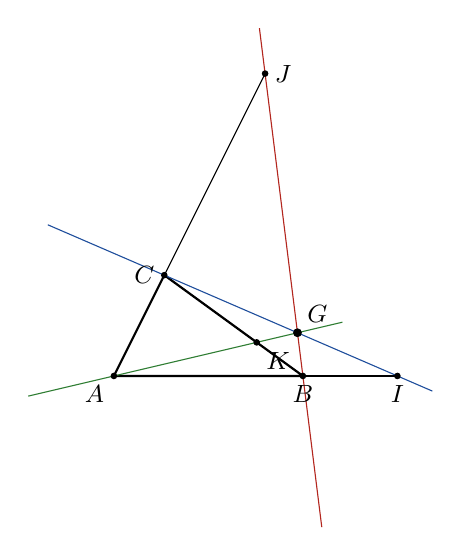
\begin{tikzpicture}[scale=0.8,font=\small]
\coordinate (A) at (0,0); \coordinate (B) at (3,0); \coordinate (C) at (0.8,1.6);
\coordinate (I) at (4.5,0); \coordinate (J) at (2.4,4.8); \coordinate (K) at (2.2667,0.5333);
\draw[thick] (A)--(B)--(C)--cycle;
\draw (B)--(I); \draw (C)--(J);
\draw[cDef] ($(C)!-0.5!(I)$)--($(C)!1.15!(I)$);
\draw[cThm] ($(B)!-0.5!(J)$)--($(B)!1.15!(J)$);
\draw[cRem] ($(A)!-0.6!(K)$)--($(A)!1.6!(K)$);
\fill (A) circle(1.5pt) node[below left]{$A$}; \fill (B) circle(1.5pt) node[below]{$B$};
\fill (C) circle(1.5pt) node[left]{$C$}; \fill (I) circle(1.5pt) node[below]{$I$};
\fill (J) circle(1.5pt) node[right]{$J$}; \fill (K) circle(1.5pt) node[below right]{$K$};
\coordinate (GG) at (2.914,0.686);
\fill[black] (GG) circle(2pt) node[above right]{$G$};
\end{tikzpicture}
\end{LTR}\end{center}
\QQ{2} $2\V{JA}-3\V{JC}=\vec0$: \bx{J\ \text{\ar{مرجح}}\ \{(A;2);(C;-3)\}} \ (و $\V{AJ}=\dfrac{-3}{-1}\V{AC}=3\V{AC}$).\par
$\V{BK}=\dfrac13\V{BC}=\dfrac{\gamma}{\beta+\gamma}\V{BC}$ مع $\beta=2$ ، $\gamma=1$: \bx{K\ \text{\ar{مرجح}}\ \{(B;2);(C;1)\}}.

\QQ{3} $2-6-3=-7\ne0$ ، فـ $G$ موجودة. نستعمل خاصية التجميع:
\begin{itemize}
\item $\{(A;2);(B;-6)\}$ متناسبة مع $\{(A;1);(B;-3)\}$ فمرجحها $I$ ، ومجموعها $-4$: \ $G$ مرجح $\{(I;-4);(C;-3)\}$ ، إذن $G\in(CI)$.
\item $\{(A;2);(C;-3)\}$ مرجحها $J$ ومجموعها $-1$: \ $G$ مرجح $\{(J;-1);(B;-6)\}$ ، إذن $G\in(BJ)$.
\item $\{(B;-6);(C;-3)\}$ متناسبة مع $\{(B;2);(C;1)\}$ فمرجحها $K$ ، ومجموعها $-9$: \ $G$ مرجح $\{(A;2);(K;-9)\}$ ، إذن $G\in(AK)$.
\end{itemize}
\textbf{الخلاصة:} \bx{(CI)\ ،\ (BJ)\ ،\ (AK)\ \text{\ar{تتلاقى في}}\ G}.
\end{hal}

% ------------------------------------------------- 11
\begin{tamrin}{استقامية ومحور قطعة}
$ABC$ مثلث ، $H$ نقطة معرفة بالعلاقة: $\V{HA}+3\V{HB}+2\V{BC}=\vec0$ ، و $G$ مرجح الجملة $\{(B;1);(C;2)\}$.
\begin{enumerate}
\item أنشئ النقطة $G$.
\item بيّن أن النقطة $H$ مرجح الجملة $\{(A;1);(B;1);(C;2)\}$ ، ثم أنشئها.
\item بيّن أن النقط $A$ ، $G$ و $H$ في استقامية.
\item $(\Gamma)$ مجموعة النقط $M$ من المستوي حيث: $\nV{\V{MB}+2\V{MC}}=\dfrac34\nV{\V{MA}+\V{MB}+2\V{MC}}$.
\begin{sq}
\qa عيّن وأنشئ المجموعة $(\Gamma)$.
\qb عيّن وأنشئ المجموعة $(\Gamma')$ حيث: $\nV{\V{MB}+2\V{MC}}\le\dfrac34\nV{\V{MA}+\V{MB}+2\V{MC}}$.
\end{sq}
\item $A(0;2)$ ، $B(-3;0)$ و $C(2;1)$ إحداثيات النقط في معلم متعامد ومتجانس.
\begin{sq}
\qa عيّن إحداثيي كل من النقطتين $G$ و $H$.
\qb تأكد حسابياً من صحة نتيجة السؤال 3.
\end{sq}
\end{enumerate}
\end{tamrin}
\begin{hal}
\textbf{1.} $\V{BG}=\dfrac{2}{1+2}\V{BC}=\bx{\dfrac23\V{BC}}$.

\QQ{2} $2\V{BC}=2\V{BH}+2\V{HC}=-2\V{HB}+2\V{HC}$ ، فتصبح العلاقة:
\[\V{HA}+3\V{HB}-2\V{HB}+2\V{HC}=\vec0\iff\bx{\V{HA}+\V{HB}+2\V{HC}=\vec0}.\]
إذن $H$ مرجح $\{(A;1);(B;1);(C;2)\}$ ، و $\V{AH}=\dfrac14\V{AB}+\dfrac12\V{AC}$.

\QQ{3} بالتجميع ($\{(B;1);(C;2)\}$ مرجحها $G$ ومجموعها $3$): \ $H$ مرجح $\{(A;1);(G;3)\}$ ، ومنه $\V{AH}=\dfrac34\V{AG}$:\par
\bx{A\ ،\ G\ ،\ H\ \text{\ar{على استقامة واحدة}}}.

\QQ{4} \pa $\V{MB}+2\V{MC}=3\V{MG}$ و $\V{MA}+\V{MB}+2\V{MC}=4\V{MH}$: \ $3MG=\dfrac34\times4MH$ ، أي $MG=MH$:\par
$(\Gamma)$ هي \bx{\text{\ar{محور القطعة}}\ [GH]}.
\pb $MG\le MH$: \ $(\Gamma')$ هي \bx{\text{\ar{نصف المستوي الذي حدّه محور}}\ [GH]\ \text{\ar{ويشمل}}\ G}.

\QQ{5} \pa $x_G=\dfrac{1(-3)+2(2)}{3}=\dfrac13$ ، $y_G=\dfrac{1(0)+2(1)}{3}=\dfrac23$: \bx{G\Big(\dfrac13;\dfrac23\Big)}.\par
$x_H=\dfrac{0-3+4}{4}=\dfrac14$ ، $y_H=\dfrac{2+0+2}{4}=1$: \bx{H\Big(\dfrac14;1\Big)}.
\pb $\V{AH}\Big(\dfrac14;-1\Big)$ و $\V{AG}\Big(\dfrac13;-\dfrac43\Big)$: \ $\dfrac14\times\Big(-\dfrac43\Big)-(-1)\times\dfrac13=-\dfrac13+\dfrac13=0$: الشعاعان مرتبطان خطياً \ok.\par
ونلاحظ أن $\V{AH}=\dfrac34\V{AG}$.
\end{hal}

% ------------------------------------------------- 12
\begin{tamrin}{تقاطع مستقيمين ودائرة}
$ABC$ مثلث كيفي ، ولتكن $I$ نقطة تحقق: $-5\V{AI}+2\V{AC}=\vec0$ ، والنقطة $H$ مرجح الجملة المثقلة $\{(A;3);(B;-2)\}$.
\begin{enumerate}
\item بيّن أن $I$ مرجح النقطتين $A$ و $C$ بمعاملين يطلب تعيينهما.
\end{enumerate}
لتكن النقطة $G$ مرجح الجملة المثقلة $\{(A;3);(B;-2);(C;2)\}$.
\begin{enumerate}[resume]
\item أثبت أن $\V{IG}=-\dfrac23\V{IB}$. استنتج أن $G$ مرجح النقطتين $B$ و $I$ بمعاملين يطلب تعيينهما.
\item بيّن أن المستقيمين $(CH)$ و $(IB)$ متقاطعان في النقطة $G$.
\item عيّن $(C_1)$ مجموعة النقط $M$ من المستوي حيث: $\nV{3\V{MA}+2\V{MC}}=0$.
\item عيّن $(C_2)$ مجموعة النقط $M$ من المستوي حيث: $\nV{3\V{MA}-2\V{MB}+2\V{MC}}=\nV{\V{MC}-\V{MB}}$.
\end{enumerate}
\end{tamrin}
\begin{hal}
\textbf{1.} $-5\V{AI}+2\big(\V{AI}+\V{IC}\big)=\vec0$ ، أي $-3\V{AI}+2\V{IC}=\vec0$ ، أي $3\V{IA}+2\V{IC}=\vec0$: \ \bx{I\ \text{\ar{مرجح}}\ \{(A;3);(C;2)\}}.

\QQ{2} $3-2+2=3\ne0$. بالتجميع ($\{(A;3);(C;2)\}$ مرجحها $I$ ومجموعها $5$): $G$ مرجح $\{(I;5);(B;-2)\}$ ، ومنه:
\[\V{IG}=\frac{-2}{5-2}\V{IB}=\bx{-\frac23\V{IB}} ,\qquad G\ \text{\ar{مرجح}}\ \{(I;5);(B;-2)\}\ \text{\ar{(أو}}\ \{(I;-5);(B;2)\}\text{\ar{)}}.\]

\QQ{3} من 2: $G\in(IB)$. \ و $H$ مرجح $\{(A;3);(B;-2)\}$ (مجموعها $1$) ، فبالتجميع: $G$ مرجح $\{(H;1);(C;2)\}$ ، إذن $G\in(CH)$.\par
المستقيمان $(CH)$ و $(IB)$ متمايزان (لأن $C\notin(IB)$) ، إذن هما \bx{\text{\ar{متقاطعان في}}\ G}.

\QQ{4} $3\V{MA}+2\V{MC}=5\V{MI}$: \ $5MI=0$ ، أي $M=I$: \ \bx{(C_1)=\{I\}}.

\QQ{5} $3\V{MA}-2\V{MB}+2\V{MC}=3\V{MG}$ ، و $\V{MC}-\V{MB}=\V{BC}$ (ثابت): \ $3MG=BC$.\par
$(C_2)$ هي \bx{\text{\ar{الدائرة التي مركزها}}\ G\ \text{\ar{ونصف قطرها}}\ \dfrac{BC}{3}}.
\end{hal}

% ------------------------------------------------- 13
\begin{tamrin}{شعاع ثابت ومرجح بوسيط $k$}
\textbf{I)} $ABC$ مثلث من المستوي. $I$ و $J$ نقطتان حيث: $\V{AI}=\dfrac34\V{AB}$ و $6\V{BJ}-2\V{CJ}=\vec0$. \ $G$ مرجح الجملة المثقلة $\{(A;1);(B;3);(C;-1)\}$.
\begin{enumerate}
\item أنشئ النقطتين $I$ و $J$ ، ثم بيّن أن $I$ مرجح للنقطتين $A$ و $B$ يطلب تعيين معاملاتهما.
\item بيّن أن $G$ نقطة تلاقي المستقيمين $(CI)$ و $(AJ)$ ، ثم أنشئ النقطة $G$.
\item بيّن أن الشعاع $\vec v=\V{MA}+3\V{MB}-4\V{MC}$ مستقل عن $M$ ، ثم بيّن أن: $\vec v=4\V{CI}$.
\item عيّن المجموعة $(\Gamma_1)$ للنقط $M$ حيث: $\nV{\V{MA}+3\V{MB}}=\nV{6\V{MB}-2\V{MC}}$.
\item عيّن المجموعة $(\Gamma_2)$ للنقط $M$ حيث: $\nV{\V{MA}+3\V{MB}-\V{MC}}=\nV{\V{MA}+3\V{MB}-4\V{MC}}$.
\end{enumerate}
\textbf{II)} لتكن $G_k$ مرجح الجملة المثقلة $\{(A;k);(B;-k);(C;1)\}$ حيث $k$ عدد حقيقي.
\begin{enumerate}[resume]
\item هل النقطة $G_k$ موجودة من أجل كل عدد حقيقي $k$؟ علّل.
\item بيّن أن: $\V{CG_k}=-k\V{AB}$ ، ثم عيّن مجموعة النقط $G_k$ لما $k$ يمسح $\R$.
\item في المعلم المتعامد والمتجانس $(O;\vec i,\vec j)$ نعتبر $A(1;2)$ ، $B(0;-2)$ و $C(-1;3)$.
\begin{sq}
\qa عيّن بدلالة $k$ إحداثيي النقطة $G_k$.
\qb عيّن قيمة $k$ حتى تنتمي $G_k$ إلى المستقيم $(D)$ الذي معادلته $y=3x$.
\end{sq}
\end{enumerate}
\end{tamrin}
\begin{hal}
\textbf{1.} $\V{AI}=\dfrac34\V{AB}=\dfrac{\beta}{\alpha+\beta}\V{AB}$ مع $\alpha=1$ ، $\beta=3$: \bx{I\ \text{\ar{مرجح}}\ \{(A;1);(B;3)\}}.\par
$6\V{BJ}-2\V{CJ}=\vec0$ تكافئ $6\V{JB}-2\V{JC}=\vec0$: $J$ مرجح $\{(B;6);(C;-2)\}$ أي $\{(B;3);(C;-1)\}$ ، و $\V{BJ}=\dfrac{-1}{2}\V{BC}$.

\QQ{2} $1+3-1=3\ne0$.
\begin{itemize}
\item $\{(A;1);(B;3)\}$ مرجحها $I$: $G$ مرجح $\{(I;4);(C;-1)\}$ ، إذن $G\in(CI)$ ، و $\V{IG}=-\dfrac13\V{IC}$.
\item $\{(B;3);(C;-1)\}$ مرجحها $J$: $G$ مرجح $\{(A;1);(J;2)\}$ ، إذن $G\in(AJ)$ ، و $\V{AG}=\dfrac23\V{AJ}$.
\end{itemize}
إذن $G$ نقطة تلاقي $(CI)$ و $(AJ)$.

\QQ{3} مجموع المعاملات $1+3-4=0$. \ بشال: $\vec v=\V{MA}+3\big(\V{MA}+\V{AB}\big)-4\big(\V{MA}+\V{AC}\big)=3\V{AB}-4\V{AC}$: \ \textbf{مستقل عن $M$}.\par
نأخذ $M=C$: $\vec v=\V{CA}+3\V{CB}=4\V{CI}$ (الاختزال بـ $I$) ، إذن \bx{\vec v=4\V{CI}}.

\QQ{4} $\V{MA}+3\V{MB}=4\V{MI}$ ، و $6\V{MB}-2\V{MC}=4\V{MJ}$: $4MI=4MJ$:\par
$(\Gamma_1)$ هي \bx{\text{\ar{محور القطعة}}\ [IJ]}.

\QQ{5} $\V{MA}+3\V{MB}-\V{MC}=3\V{MG}$ و $\nV{\vec v}=4CI$: \ $3MG=4CI$ ، أي $MG=\dfrac43CI$:\par
$(\Gamma_2)$ هي \bx{\text{\ar{الدائرة التي مركزها}}\ G\ \text{\ar{ونصف قطرها}}\ \dfrac43CI}.

\QQ{6} $k-k+1=1\ne0$ من أجل كل $k$: \ \textbf{نعم} ، $G_k$ موجودة من أجل كل $k\in\R$.

\QQ{7} $k\V{G_kA}-k\V{G_kB}+\V{G_kC}=\vec0$ ، أي $k\V{BA}+\V{G_kC}=\vec0$ ، ومنه $\V{CG_k}=k\V{BA}=\bx{-k\V{AB}}$.\par
لما $k$ يمسح $\R$: مجموعة النقط $G_k$ هي \bx{\text{\ar{المستقيم الذي يشمل}}\ C\ \text{\ar{ويوازي}}\ (AB)}.

\QQ{8} \pa $x_{G_k}=\dfrac{k(1)-k(0)+1(-1)}{1}=k-1$ ، \ $y_{G_k}=\dfrac{2k+2k+3}{1}=4k+3$: \bx{G_k(k-1;4k+3)}.
\pb $4k+3=3(k-1)\iff4k+3=3k-3\iff\bx{k=-6}$ ، و $G_{-6}(-7;-21)$.
\end{hal}
\begin{molahada}
في أحد الحلول المتداولة لهذا التمرين كُتب نصف القطر $\dfrac34CI$ ، والصحيح $\dfrac43CI$ (من $3MG=4CI$).
\end{molahada}

% ------------------------------------------------- 14
\begin{tamrin}{مجموعة نقط بتوظيف دراسة دالة}
$ABC$ مثلث و $m$ عدد حقيقي من المجال $[-1;1]$. \ نعتبر $G_m$ مرجح الجملة المثقلة $\{(A;m^2+1);(B;m);(C;-m)\}$.
\begin{enumerate}
\item برّر وجود $G_m$ من أجل كل عدد حقيقي $m$ من المجال $[-1;1]$ ، ثم بيّن أن: $\V{AG_m}=\dfrac{-m}{m^2+1}\V{BC}$.
\item أنشئ النقطتين $G_1$ و $G_{-1}$.
\item لتكن $N$ نقطة من $(BC)$. هل يمكن أن تنطبق $N$ على $G_m$؟ علّل.
\item شكّل جدول تغيرات الدالة $f$ المعرفة على $[-1;1]$ بـ: $f(x)=\dfrac{-x}{x^2+1}$.
\item استنتج مجموعة النقط $G_m$ عندما يمسح $m$ المجال $[-1;1]$.
\end{enumerate}
\end{tamrin}
\begin{hal}
\textbf{1.} مجموع المعاملات: $m^2+1+m-m=m^2+1\ge1>0$: $G_m$ موجودة.
\[\V{AG_m}=\frac{m\V{AB}-m\V{AC}}{m^2+1}=\frac{m\big(\V{AB}+\V{CA}\big)}{m^2+1}=\frac{m\V{CB}}{m^2+1}=\bx{\frac{-m}{m^2+1}\V{BC}}.\]
\QQ{2} $m=1$: $\V{AG_1}=-\dfrac12\V{BC}$ ؛ \quad $m=-1$: $\V{AG_{-1}}=\dfrac12\V{BC}$. \ (النقطتان متناظرتان بالنسبة لـ $A$.)
\QQ{3} $\V{AG_m}$ و $\V{BC}$ مرتبطان خطياً ، فـ $G_m$ تنتمي إلى المستقيم $(\Delta)$ الذي يشمل $A$ ويوازي $(BC)$.\par
$(\Delta)\parallel(BC)$ و $A\notin(BC)$ ، فهما متوازيان تماماً ولا يتقاطعان: \bx{N\ \text{\ar{لا يمكن أن تنطبق على}}\ G_m}.
\QQ{4} $f'(x)=\dfrac{-(x^2+1)-(-x)(2x)}{(x^2+1)^2}=\dfrac{x^2-1}{(x^2+1)^2}\le0$ على $[-1;1]$: $f$ متناقصة.
\begin{TAB}
\tkzTabInit[lgt=1.3,espcl=3]{$x$/0.7,$f'(x)$/0.7,$f(x)$/1.3}{$-1$,$1$}
\tkzTabLine{z,-,z}
\tkzTabVar{+/$\frac12$,-/$-\frac12$}
\end{TAB}
\QQ{5} $\V{AG_m}=f(m)\V{BC}$ و $f(m)$ يمسح المجال $\Big[-\dfrac12;\dfrac12\Big]$ لما $m$ يمسح $[-1;1]$:\par
مجموعة النقط $G_m$ هي \bx{\text{\ar{القطعة المستقيمة}}\ [G_{-1}G_1]} \ (منتصفها $A$ ، وهي موازية لـ $(BC)$).
\end{hal}

% =====================================================================
\section{مجموعات النقط}
% ------------------------------------------------- 15
\begin{tamrin}{مثلث متقايس الأضلاع}
$ABC$ مثلث متقايس الأضلاع حيث $AB=AC=BC=2$. \ لتكن $(\Gamma)$ مجموعة النقط $M$ من المستوي التي تحقق:
\[\nV{\V{MA}-4\V{MB}+\V{MC}}=\nV{\V{MA}-2\V{MB}+\V{MC}}.\]
\begin{enumerate}
\item تحقق أن النقطة $B$ تنتمي إلى $(\Gamma)$.
\item بيّن أن الشعاع $\V{MA}-2\V{MB}+\V{MC}$ مستقل عن النقطة $M$.
\item ليكن $G$ مرجح الجملة المثقلة $\{(A;1);(B;-4);(C;1)\}$. بيّن أن $GM=\sqrt3$ من أجل كل $M\in(\Gamma)$.
\item استنتج طبيعة المجموعة $(\Gamma)$ محدداً عناصرها المميزة ، ثم أنشئها.
\end{enumerate}
\end{tamrin}
\begin{hal}
\textbf{1.} $M=B$: الطرف الأيسر: $\nV{\V{BA}+\V{BC}}$ ، والطرف الأيمن: $\nV{\V{BA}+\V{BC}}$: متساويان ، إذن \bx{B\in(\Gamma)}.
\QQ{2} مجموع المعاملات $1-2+1=0$: \ $\V{MA}-2\V{MB}+\V{MC}=\big(\V{MA}-\V{MB}\big)+\big(\V{MC}-\V{MB}\big)=\bx{\V{BA}+\V{BC}}$ (ثابت).
\QQ{3} $1-4+1=-2$: $\V{MA}-4\V{MB}+\V{MC}=-2\V{MG}$ ، فالشرط: $2MG=\nV{\V{BA}+\V{BC}}$.\par
لتكن $I$ منتصف $[AC]$: $\V{BA}+\V{BC}=2\V{BI}$ ، و $BI$ ارتفاع المثلث المتقايس الأضلاع: $BI=\sqrt{2^2-1^2}=\sqrt3$.\par
إذن $2MG=2\sqrt3$ ، أي \bx{GM=\sqrt3}.
\QQ{4} $(\Gamma)$ هي \bx{\text{\ar{الدائرة التي مركزها}}\ G\ \text{\ar{ونصف قطرها}}\ \sqrt3}.\par
\textbf{إنشاء $G$:} $\V{AG}=\dfrac{-4\V{AB}+\V{AC}}{-2}=2\V{AB}-\dfrac12\V{AC}$ ، أو بالتجميع: $G$ مرجح $\{(I;2);(B;-4)\}$ ، أي $\V{BG}=-\V{BI}$: $G$ نظيرة $I$ بالنسبة لـ $B$.\par
(ونتحقق: $GB=BI=\sqrt3$ ، فعلاً $B\in(\Gamma)$.)
\begin{center}\begin{LTR}
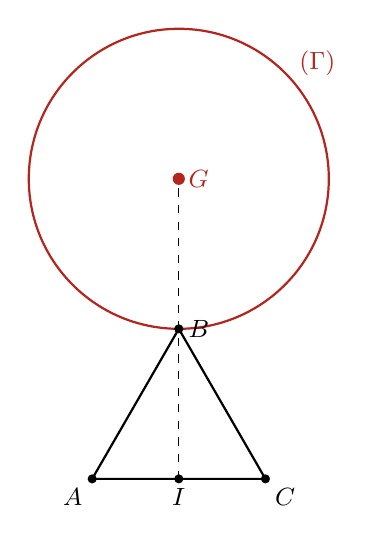
\begin{tikzpicture}[scale=1.1,font=\small]
\coordinate (A) at (-1,0); \coordinate (C) at (1,0); \coordinate (B) at (0,1.732);
\coordinate (I) at (0,0); \coordinate (G) at (0,3.464);
\draw[thick] (A)--(B)--(C)--cycle; \draw[dashed] (I)--(G);
\draw[cThm,thick] (G) circle(1.732);
\fill (A) circle(1.5pt) node[below left]{$A$}; \fill (C) circle(1.5pt) node[below right]{$C$};
\fill (B) circle(1.5pt) node[right]{$B$}; \fill (I) circle(1.5pt) node[below]{$I$};
\fill[cThm] (G) circle(2pt) node[right]{$G$}; \node[cThm] at (1.6,4.8){$(\Gamma)$};
\end{tikzpicture}
\end{LTR}\end{center}
\end{hal}

% ------------------------------------------------- 16
\begin{tamrin}{تطبيق فيزيائي: مركز الثقل (تمرين نموذجي)}
\begin{enumerate}
\item قضيب متجانس $[AB]$ كتلته مهملة وطوله $1{,}2\ \text{m}$. نعلّق كتلة $2\ \text{kg}$ في الطرف $A$ وكتلة $4\ \text{kg}$ في الطرف $B$. \ نعلم أن نقطة التوازن (مركز الثقل) $G$ هي مرجح $\{(A;2);(B;4)\}$. \ أين نعلّق القضيب حتى يبقى متوازناً؟
\item نضيف كتلة $3\ \text{kg}$ في منتصف القضيب $I$. عيّن الموضع الجديد لنقطة التوازن.
\item صفيحة رقيقة كتلتها مهملة على شكل مثلث $ABC$ ، حيث $A(0;0)$ ، $B(6;0)$ و $C(0;3)$ (الوحدة: dm). نضع كتلاً $1\ \text{kg}$ في $A$ ، $2\ \text{kg}$ في $B$ و $3\ \text{kg}$ في $C$. \ عيّن إحداثيي نقطة توازن الصفيحة.
\end{enumerate}
\end{tamrin}
\begin{hal}
\textbf{1.} $\V{AG}=\dfrac{4}{2+4}\V{AB}=\dfrac23\V{AB}$: \ $AG=\dfrac23\times1{,}2=\bx{0{,}8\ \text{m}}$ من الطرف $A$ (أقرب إلى الكتلة الأثقل).
\QQ{2} $G'$ مرجح $\{(A;2);(B;4);(I;3)\}$. بالتجميع: $G'$ مرجح $\{(G;6);(I;3)\}$ ، ومنه $\V{GG'}=\dfrac{3}{9}\V{GI}=\dfrac13\V{GI}$.\par
$AI=0{,}6$ و $AG=0{,}8$ ، فـ $GI=0{,}2$ (في اتجاه $A$) ، و $AG'=0{,}8-\dfrac{0{,}2}{3}\approx\bx{0{,}733\ \text{m}}$ من $A$.\par
(تحقق مباشر على محور: $x_{G'}=\dfrac{2\times0+4\times1{,}2+3\times0{,}6}{9}=\dfrac{6{,}6}{9}\approx0{,}733$ \ok.)
\QQ{3} $x=\dfrac{1\times0+2\times6+3\times0}{6}=2$ ، \ $y=\dfrac{0+0+3\times3}{6}=1{,}5$: \ نقطة التوازن \bx{(2;1{,}5)}.
\end{hal}

% =====================================================================
\section{الاختيار من متعدد وصحيح أم خطأ}
% ------------------------------------------------- 17
\begin{tamrin}{اختيار من متعدد}
عيّن الاقتراح الصحيح الوحيد في كل حالة مع التعليل:
\begin{enumerate}
\item $G$ مرجح $\{(A;2);(B;-1)\}$. \ لدينا:
\ABC{$\V{AG}=-\V{AB}$}{$\V{AG}=\V{AB}$}{$\V{AG}=2\V{AB}$}
\item الجملة المثقلة $\{(A;3);(B;-3)\}$:
\ABC{مرجحها منتصف $[AB]$}{ليس لها مرجح}{مرجحها $A$}
\item $G$ مركز ثقل المثلث $ABC$. من أجل كل نقطة $M$: $\V{MA}+\V{MB}+\V{MC}$ يساوي:
\ABC{$\V{MG}$}{$3\V{MG}$}{$\vec0$}
\item $A(0;0)$ ، $B(3;0)$ و $C(0;6)$. مرجح $\{(A;1);(B;2);(C;3)\}$ هو:
\ABC{$(1;3)$}{$(3;1)$}{$(1;2)$}
\item مجموعة النقط $M$ حيث $\nV{\V{MA}+\V{MB}}=AB$ هي:
\ABC{دائرة قطرها $[AB]$}{محور $[AB]$}{دائرة مركزها $A$}
\item مجموعة النقط $M$ حيث $\nV{2\V{MA}-\V{MB}-\V{MC}}=4$ ($ABC$ مثلث) هي:
\ABC{دائرة}{المستوي كله أو المجموعة الخالية}{مستقيم}
\end{enumerate}
\end{tamrin}
\begin{hal}
\textbf{1.} (أ): $\V{AG}=\dfrac{-1}{2-1}\V{AB}=\bx{-\V{AB}}$.
\QQ{2} (ب): مجموع المعاملين $3-3=0$: \bx{\text{\ar{لا يوجد مرجح}}}.
\QQ{3} (ب): $G$ مرجح $\{(A;1);(B;1);(C;1)\}$ ، فبالاختزال: \bx{\V{MA}+\V{MB}+\V{MC}=3\V{MG}}.
\QQ{4} (أ): $x=\dfrac{0+6+0}{6}=1$ ، $y=\dfrac{0+0+18}{6}=3$: \bx{(1;3)}.
\QQ{5} (أ): $\V{MA}+\V{MB}=2\V{MI}$ ($I$ منتصف $[AB]$): $2MI=AB$ ، أي $MI=\dfrac{AB}{2}$: \bx{\text{\ar{الدائرة التي قطرها}}\ [AB]}.
\QQ{6} (ب): مجموع المعاملات $0$: الشعاع ثابت $\vec u=\V{BA}+\V{CA}$. \ إذا كان $\|\vec u\|=4$ فكل نقط المستوي تحقق الشرط ، وإلا فلا توجد أي نقطة: \bx{\text{\ar{المستوي كله أو}}\ \varnothing}.
\end{hal}

% ------------------------------------------------- 18
\begin{tamrin}{صحيح أم خطأ}
أجب بصحيح أو خطأ مع التبرير:
\begin{enumerate}
\item إذا كانت $G$ مرجح $\{(A;\alpha);(B;\beta)\}$ حيث $\alpha>0$ و $\beta>0$ فإن $G\in[AB]$.
\item مرجح $\{(A;2);(B;6)\}$ هو نفسه مرجح $\{(A;1);(B;3)\}$.
\item الجملة المثقلة $\{(A;1);(B;1);(C;-2)\}$ تقبل مرجحاً.
\item إذا كانت $G$ مرجح $\{(A;1);(B;1);(C;2)\}$ و $I$ منتصف $[AB]$ فإن $G$ منتصف $[IC]$.
\item $\{(A;1);(B;-2)\}$ مرجحها $K$ و $I$ منتصف $[AB]$. مجموعة النقط $M$ حيث $\nV{\V{MA}-2\V{MB}}=\nV{\V{MA}+\V{MB}}$ هي محور $[KI]$.
\end{enumerate}
\end{tamrin}
\begin{hal}
\textbf{1. صحيح:} $\V{AG}=\dfrac{\beta}{\alpha+\beta}\V{AB}$ و $0<\dfrac{\beta}{\alpha+\beta}<1$.
\QQ{2} \textbf{صحيح:} خاصية التجانس ($k=2$) ، وفي الحالتين $\V{AG}=\dfrac34\V{AB}$.
\QQ{3} \textbf{خطأ:} $1+1-2=0$.
\QQ{4} \textbf{صحيح:} بالتجميع $G$ مرجح $\{(I;2);(C;2)\}$.
\QQ{5} \textbf{خطأ:} $\V{MA}-2\V{MB}=-\V{MK}$ و $\V{MA}+\V{MB}=2\V{MI}$ ، فالشرط هو $MK=2MI$ وليس $MK=MI$.\par
مثلاً منتصف $[KI]$ ينتمي إلى محور $[KI]$ لكنه لا يحقق $MK=2MI$.
\end{hal}

\end{document}
